%!TEX root = thesis.tex

\documentclass[a4paper]{article}
\usepackage{amsthm}
\usepackage[utf8]{inputenc}
\usepackage{csquotes}
\usepackage[english]{babel}
\usepackage{graphicx}
\usepackage{enumitem}
\usepackage{subcaption}  %ALLOWS SUBFIGURES
\usepackage{wrapfig}

\usepackage[draft]{fixme}
\fxsetup{theme = color}
\definecolor{fxnote}{rgb}{0.0000, 0.6000,0.0000}
\definecolor{fxwarning}{rgb}{1.0000,0.5490,0.0000}
\definecolor{fxerror}{rgb}{1.0000,0.2706,0.0000}
\definecolor{fxfatal}{rgb}{1.0000,0.0000,0.0000}
\usepackage[backend=biber, giveninits =true, isbn=false, url=false, maxbibnames=100]{biblatex}
\usepackage{hyperref}

%Theorems
\newtheorem{thrm}{Theorem}
\newtheorem{lemma}[thrm]{Lemma}
\newtheorem{prop}[thrm]{Proposition}
\newtheorem{remark}[thrm]{Remark}

\theoremstyle{definition}
\newtheorem*{defi}{Definition}

%%BeginIpePreamble
\usepackage{amsmath}
\usepackage{amssymb}
\usepackage{amsopn}

\newcommand{\scr}[1]{\mathcal{#1}}
\newcommand{\Z}{\mathbb{Z}}
\newcommand{\F}{\mathbb{F}}
\newcommand{\R}{\mathbb{R}}
\newcommand{\N}{\mathbb{N}}
\newcommand{\Q}{\mathbb{Q}}


%Operators
\newcommand{\id}{\operatorname{Id}}



%braces etc
\newcommand{\braces}[1]{\left\lbrace {#1} \right\rbrace}
\newcommand{\sqbr}[1]{\left\lbrack {#1} \right\rbrack }
\newcommand{\abs}[1]{\left\lvert {#1} \right\rvert }
\newcommand{\ceil}[1]{\left\lceil{ #1 } \right\rceil}
\newcommand{\floor}[1]{\left \lfloor {#1}\right\rfloor}
\newcommand{\parens}[1]{\left( {#1} \right)}


%utility
\newcommand{\inv}[1]{{#1}^{-1}}
\newcommand{\half}{\frac{1}{2}}
\newcommand{\third}{\frac{1}{3}}
\newcommand{\goes}{\rightarrow}
\newcommand{\nin}{\not \in}
\newcommand{\sm}[1]{\setminus \braces{#1} }

%vectors and matrices
\newcommand{\zerov}{\vec{0}}
\newcommand{\onev}{\vec{1}}

\newcommand{\twovec}[2]{\parens{ \begin{array}{c}#1 \\ #2\end{array} }}
\newcommand{\threevec}[3]{\prens{ \begin{array}{c}#1 \\ #2\\#3 \end{array} }}
\newcommand{\fourvec}[4]{\parens{ \begin{arr\newcommand{\ifftext}{if and only if }ay}{c}#1 \\ #2\\#3\\#4 \end{array} }}
\newcommand{\twomatrix}[4]{\parens{\begin{array}{cc}#1 & #2 \\ #3 & #4 \end{array}  }}
\newcommand{\twodiagmatrix}[2]{\parens{\begin{array}{cc}#1 & 0 \\ 0 & #2 \end{array}  }}

%%%%THIS THESIS
\newcommand{\intplus}{\operatorname{Int^{+}}}
\newcommand{\interior}{\operatorname{Int}}
\newcommand{\spl}{\operatorname{split}}
\newcommand{\mrg}{\operatorname{merge}}


\newcommand{\ext}[1]{\bar{#1}}
\newcommand{\tightext}[1]{\bar{#1}_t}
\newcommand{\dualgraph}[1]{\G(#1)}
\newcommand{\extdualgraph}[1]{\G_{\scr E}(#1)}



\newcommand{\W}{\scr W}
\renewcommand{\P}{\scr P}
\newcommand{\C}{\scr C}
\newcommand\restrict[1]{\raisebox{-.5ex}{$|$}_{#1}}
\newcommand{\restC}[1]{\ensuremath{\C\restrict{#1}}}

%p is for pole
\newcommand{\pN}{\mathrm{N}}
\newcommand{\pS}{\mathrm{S}}
\newcommand{\pE}{\mathrm{E}}
\newcommand{\pW}{\mathrm{W}}

\newcommand{\cpath}{\C \setminus \braces{\pS}} %cycle path

\newcommand{\rel}{\text{regular edge labeling }}

%%EndIpePreamble


%bib stuff
\bibstyle{plain}



\begin{document}
\maketitle

\section{Types of triangulations and their properties}
\subsection{Preliminaries}
All graphs are presumed simple and have a fixed planar embedding. In this thesis paths and cycles are always simple while walks are not necessarily simple.

The \emph{degree} of a face is the number of vertices it is incident to. By a \emph{cycle} we will mean a simple cycle. That is a cycle without repetition of edges or vertices. By Jordan's curve theorem a cycle splits the plane into two parts, one bounded and one unbounded. %TODO cite 
We will call the bounded part the \emph{interior} of this cycle and the unbounded part the \emph{exterior} of this cycle.

We will call a cycle \emph{separating} if there are vertices in both it's interior and exterior. We will use \emph{$k$-cycle} to denote a cycle of length $k$. Moreover a \emph{triangle} is simply a cycle of length $3$ (i.e. a $3$-cycle). 


\subsection{Plane triangulations}

\begin{defi} [Plane triangulation]
A graph with only faces of degree $3$.
\end{defi}


\begin{defi} [Maximal planar graph]
A graph such that adding any one edge leaves it non-planar.
\end{defi}

\begin{thrm}
Any graph $G$ is a plane triangulation \ifftext it is maximal planar
\end{thrm}

\begin{proof}
We will prove the equivalence of the negations.

Suppose that $G$ is not maximally planar. Then there is a face $F$ to which we can add an edge, however this face must then have degree larger then $4$. Hence $G$ is also not a plane triangulation. 

Suppose that $G$ is not a plane triangulation. Then there must be a face $F$ of degree larger then $3$. This face will thus admit an extra edge without violating planarity and hence $G$ is not maximally planar.
\end{proof}

\subsubsection{Connectedness}
\begin{thrm}
Any plane triangulation $T$ is $3$-connected.
\label{th:plTri3Connected}
\end{thrm}

\begin{proof}
Suppose that $T$ is not $3$-connected. Then there must be a $2$-cutset $S$, given by the vertices $x$ and $y$. Removing this cutset splits the graph into at least two connected components $C_i$ and all components are incident to all cutvertices otherwise we would have found a $1$-cutset.

Since $S$ is a cutset, there can't be any edges incident to both $C_1$ and $C_2$. But then the edge $xy$ should be separating the $2$ components on both sides. This is impossible since we can only draw this edge once. %TODO figure/ and clarify
\end{proof}

\begin{defi}[Irreducible triangulation]
We call a triangulation irreducible if it has no separating triangles
\end{defi}

%TODO show reduction?

\begin{thrm}
Any irreducible plane triangulation $T$ is $4$-connected.
\end{thrm}

\begin{proof}
Note that any plane triangulation is $3$-connected by Theorhem \ref{th:plTri3Connected}.

Suppose that $T$ is not $4$-connected. Then there must be some $3$-cutset (since it is $3$-connected) let us denote the vertices of this cutset by $x, y$ and $z$. Removing this cutset splits the graph into at least two connected components $C_i$ and all components are incident to all cutvertices otherwise we would have found a $2$- or $1$-cutset.  

However, now $xy$ must be an edge in the triangulation $T$ otherwise the graph is not maximal planar (There can't be an edge incident to both $C_1$ and $C_2$ because that would negate $x, y ,z$ being a cutset.). In the same way $yz$ and $xz$ are edges of $T$. But then $xyz$ is a separating triangle. This is an contradiction and thus $T$ is $4$-connected
\end{proof}

\subsection{Triangulations of the $k$-gon}

\begin{defi}[Triangulation of the $k$-gon]
We call a graph a triangulation of the $k$-gon if the outer face has degree $k$ and all interior faces have degree $3$.
\end{defi}
Vertices bordering the outer face are \emph{outer vertices} while all other vertices are \emph{interior vertices}. Furthermore the cycle formed by all vertices outer vertices is the \emph{outer cycle}.

Sometimes such triangulations of the $k$-gon are called \emph{(plane) triangulated graphs}.


\begin{defi}[Irreducible triangulation of the $k$-gon]
We call a triangulation of the $k$-gon irreducible if it has no separating triangles.
\end{defi}


Note that triangulation of the $n$-gon $n\geq 4$ is not maximally planar and thus not plane triangulation.

\begin{comment}
%Don't know yet if this a usfull construct
\begin{thrm}
The interior of a triangulation of the $n$-gon is maximally planar. That is to say, we can't add any edges except trough the outer face.
\end{thrm}

\begin{proof}
Suppose the 
%TODO (not max plan. => face of degree 4
\end{proof}
\end{comment}

The \emph{completion} of a triangulation of the $k$-gon $G = (V, E)$. Is the graph $G'= (V', E')$ with vertex set $V' = V \cup \braces{s}$ and edge set $E' = E \cup \braces{ sv | v \text{ is a outer vertex}}$ 

The completion is plane triangulation.  %Q does this stament need proof? 
Since the interior of the outer cycle of $G$ always consisted of faces of degree 3. The exterior of the outer cycle consisted of one face of degree $k$ (the outer face) but the completion has turned this into $k$ faces of degree $3$.  

\begin{thrm}
A triangulation of the $k$-gon $G$ is $2$-connected.
\end{thrm}
\begin{proof}
Suppose that $G$ has a cutvertex $v$. Then the set $\braces{s, v}$ is a $2$-cutset of the completion $G'$ of $G$. This however is in contradiction to Theorem \ref{th:plTri3Connected} stating that $G'$ is $3$-connected. Hence $G$ has no cutvertex and is thus $2$-connected.
\end{proof}

\begin{thrm}
\label{th:irreducible and chordless triangulation of the kgon is 3connected}
A irreducible and chordless triangulation of the $k$-gon is $3$-connected.
\end{thrm}
\begin{proof}
\note Will be provided if this statement turns out to be interesting. Will go via the fact that the completion is a irreducible triangulation. Chordless outer cycle is important, because a chord will form a separating triangle in $G'$.
\end{proof}

\begin{thrm}
Any irreducible triangulation $T$ of the $4$-gon with $n \geq 5$ is $3$-connected. 
\end{thrm}

\note This proof could be a corrolary of the above theorhem \ref{th:irreducible and chordless triangulation of the kgon is 3connected}. A chord gives a separating triangle if $n\geq 5$.
\begin{proof} 
Let us name the four outer vertices $a,b,c,d$ in clockwise order. Let us first note that the diagonals $ac$ and $bd$ can't be an edge since this would create a separating triangle containing the $5$th vertex. Let $I$ denote the component of all interior vertices, since every face in the interior is of degree $3$ each outer vertices is incident to at least one edge that is also incident to $I$. %TODO figure

One can now easily check that there is no $2$cut set with only exterior vertices. However, a cutset with $1$ or $2$ interior vertices leads to at least one cycle of degree greater then $3$ %TODO expand/ figure.

Hence no $2$-cutset of $T$ can't exist and $T$ is $3$-connected. 
\end{proof}

\begin{thrm}
For every interior vertex $v$ of a triangulation of the $k$-gon $G$ is connected by ate least $3$ vertex disjoint paths to different outer vertices.
\end{thrm}
\begin{proof}
By Theorhem \ref{th:plTri3Connected} the completion $G'$ of $G$ is $3$-connected. Hence there are 3 vertex-disjoint paths from $v$ to $s$. Since $v$ is on the interior and $s$ is on the exterior of the outer cycle $\C$ all these 3 paths cross the outer cycle at least once. These paths cross $\C$ for the first time in different vertices since they are vertex-disjoint. If we shorten the paths to their first crossing with $\C$ we obtain the $3$ paths in the theorem.
\end{proof}

\note We can sharpen this to $4$ if we have a irreducible an chordless triangulation of the $k$-gon

\begin{thrm} 
Every interior vertex of a triangulation of the $n$-gon has degree at least $3$.
\end{thrm}
\begin{proof}
Suppose a interior vertex $v$ has degree $1$ then clearly the face surrounding $v$ can't have degree $3$. Now suppose that an interior vertex $v$ has degree $2$. We then let $u$ and $w$ denote it's neighbours and $F$ and $F'$ the face incident to $v$. See also Figure \ref{fig:interiorVertexDegree3}. Then since $F$ and $F'$ are both interior faces they need to be off degree $3$ this implies that $uw$ is an edge for both faces. This is impossible and hence every interior vertex has at least degree $3$
\end{proof}

\begin{figure}[h!]
\centering
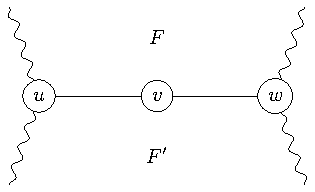
\includegraphics{img/interiorVertexDegree3.pdf}
\caption{The notation as described in the proof \label{fig:interiorVertexDegree3}
}
\end{figure}

\note If we forbid irreducible triangulations every interior vertex is of degree $4$ since the neighbourhood of any internal vertex $v$ looks like a set of triangles.

\note This theorem is currently (17-09) unused.




\section{Rectangular duals}

\newcommand{\G}{\scr G}
\renewcommand{\L}{\scr L}

In this section we will explain what we mean with the rectangualr dual of a graph. We will prove some simple properties of graphs and their duals.

We define a \emph{rectangular layout} (or simply \emph{layout}) $\L$ to be a partition of a rectangle into finitely many interiorly disjoint rectangles. 

We will assume that no four rectangles meet in one point.

We will then look at the \emph{dual graph of a layout} $\L$ and denote this graph by $\G(\L)$. That is, we represent each rectangle by a vertex and we connect two vertices by an edge exactly when their rectangles are adjacent. Note that this graph is not the same as the \emph{graph dual} of $\L$ when we view it as a graph (namely we don't represent the outer face of $\L$ by a vertex).

So $\G(\L)$ is the dual graph of a layout $\L$. In the reverse direction we say a layout $\L$ is a \emph{rectangular dual} of a graph $\G$ if we have that $\G = \G (\L)$.

A plane triangulated graph $\G$ does not necessarily have a rectangular dual nor is this dual necessarily unique.
%TODO in what sense not unique
%TODO provide examples

%TODO weave a corner assignment in here somewhere

\subsection{Extended graphs}
A \emph{extended graph} $\ext G$ of $G$ is a augmentation of $G$ with $4$  vertices (which we will call it's \emph{poles}). Such that 
\begin{enumerate}
\item every interior face has degree $3$ and the exterior face has degree $4$.
\item all poles are incident to the outer face
\item $\ext\G$ has no separating triangles (i.e separating $3$-cycles).
\end{enumerate}.

We sometimes call an extended graph $\ext G$ of $G$ an \emph{extension} of $G$.

Such a extended graph does not necessarily exist and is not necessarily unique.  %TODO show this
However we have the following result due to .... %TODO cite

\begin{thrm}[Existence of a rectangular dual]
A plane triangulated graph $\G$ has a rectangular dual \ifftext it has an extension $\ext \G$
\end{thrm}

\begin{proof}
Kozminski \& kinnen and ungar, See siAM paper %TODO check this
\end{proof}

We call any (plane triangulated) graph $G$ that has an extension a \emph{proper} graph.

A proper graph $G$ can have more then one extensions. Each such extension fixes which of the rectangles are in the corners of the rectangular dual $\L$. Hence sometimes such an extension is called a \emph{corner assignment}.


\subsection{Regular edge labeling}
A regular edge labelling  of $\ext G$ corresponds to a rectangular dual $\L$ of $G$ with some \emph{corner assignment} fixed. %TODO KANT HE
%explain equivalence

Or regular edge labelling of a graph.


An \emph{interior edge} of a cycle is an edge on the interior of the cycle (when the cycle is viewed as Jordan curve).


\subsubsection{Being onesided in terms of REL}

\subsubsection{Being psudeo-onesided in terms of REL}

\section{Fixing a extension}
In our explorations to find a lower bound on what kind of \emph{psuedo one-sidedness} is possible we will find it very useful to fix one particular extension $\ext G$ of $G$. Unfortunately if there is no rectangular dual that’s $(k,l)$-sided using the \emph{corner assignment} provided by some extension $\ext G$. This does not imply that $G$ is not $(k,l)$-sided. There might be another extension of $G$ such that under the corner assignment corresponding to this extension $G$ has a $(k,l)$-sided rectangular dual. 

Fortunately for us however we can view $\ext G = H$ as a graph in it's own right, then $G$ is the interior of a separating $4$-cycle of $H$ and we will show this implies that $G$ (as induced sugraph) has to be coloured according to the extension $\ext G$. 

\begin{remark}
\label{re:interiorRectangle}
Let $\C$ be a separating $4$-cyle of $G$ with interior $I$. Then in any rectangular dual of $G$ the region enclosed by the rectangles dual to the vertices in $\C$ is a rectangle.
\end{remark}

\begin{remark}
\label{re:disjointRectanglesOnlyHaveOneAdjecentSide}
Two disjoint rectangles are at most adjacent on one side.
\end{remark}

\begin{lemma}
\label{lem:fourCycleUnicolor}
Let $\C = \braces{a, b, c, d}$ be a separating $4$-cyle of $\ext G$ with interior $I$. Then all interior edges incident to $a, b, c$ and $d$ respectively are red, blue, red and blue or blue, red, blue and red.
\end{lemma}

\begin{proof}
%from page 4
%We could also try a reduction along the lines of min. seperation componenets Epstein et. al
By Remark \ref{re:interiorRectangle} the union of the rectangles in the interior of $\C$ will be some rectangle in any rectangular dual. We will denote this rectangle by $I$. Since two disjoint rectangles can only be adjacent to each other at one side all interior edges incident to any vertex of $\C$ are of the same color. 

Furthermore $a, b, c, d$ are all adjacent to a different side of $I$ since $I$ has four sides that need to be covered and it is only adjacent to four rectangles. If we then apply the rules of a regular edge labelling we see that if the interior edges of $a$ are one color, those incident to $b$ and $d$ should have the second color. Then of course the interior edges incident to $c$ are again coloured with the first color. 

\end{proof}

This lemma implies that any \emph{alternating 4-cycle} %TODO define
is either \emph{left-alternating} or \emph{right-alternating} %TODO define
in the terminology of \Fusy

Furthermore the above Lemma is also very useful in that it allows us to fix a extension $\ext G$ of $G$ by building a \emph{scaffold}. Suppose we want to investigate some extension $\ext G$ of $G$ with poles $N$, $E$, $S$ and $W$ then we can consider the graph $\ext G = H$ as a graph in it's own right. $H$ is a proper graph since it has no irreducible triangles in it's interior (because $\ext G$ had none) and it admits a valid extension $\ext H$ by connecting the new poles $NE, SE, SW$ and $NW$ to $N, E, SE, NW$, $S, E, NE, SW$, $S, W, SE, NW$ and $N, W, NE, SW$ respectively. See Figure \ref{fig:scafold} for this extension.  
\fxnote{Maybe use a table}

\begin{thrm}
\label{th:fixExtension}
We can fix an extension, if we want.
\end{thrm}

\begin{figure}[h!]
\centering
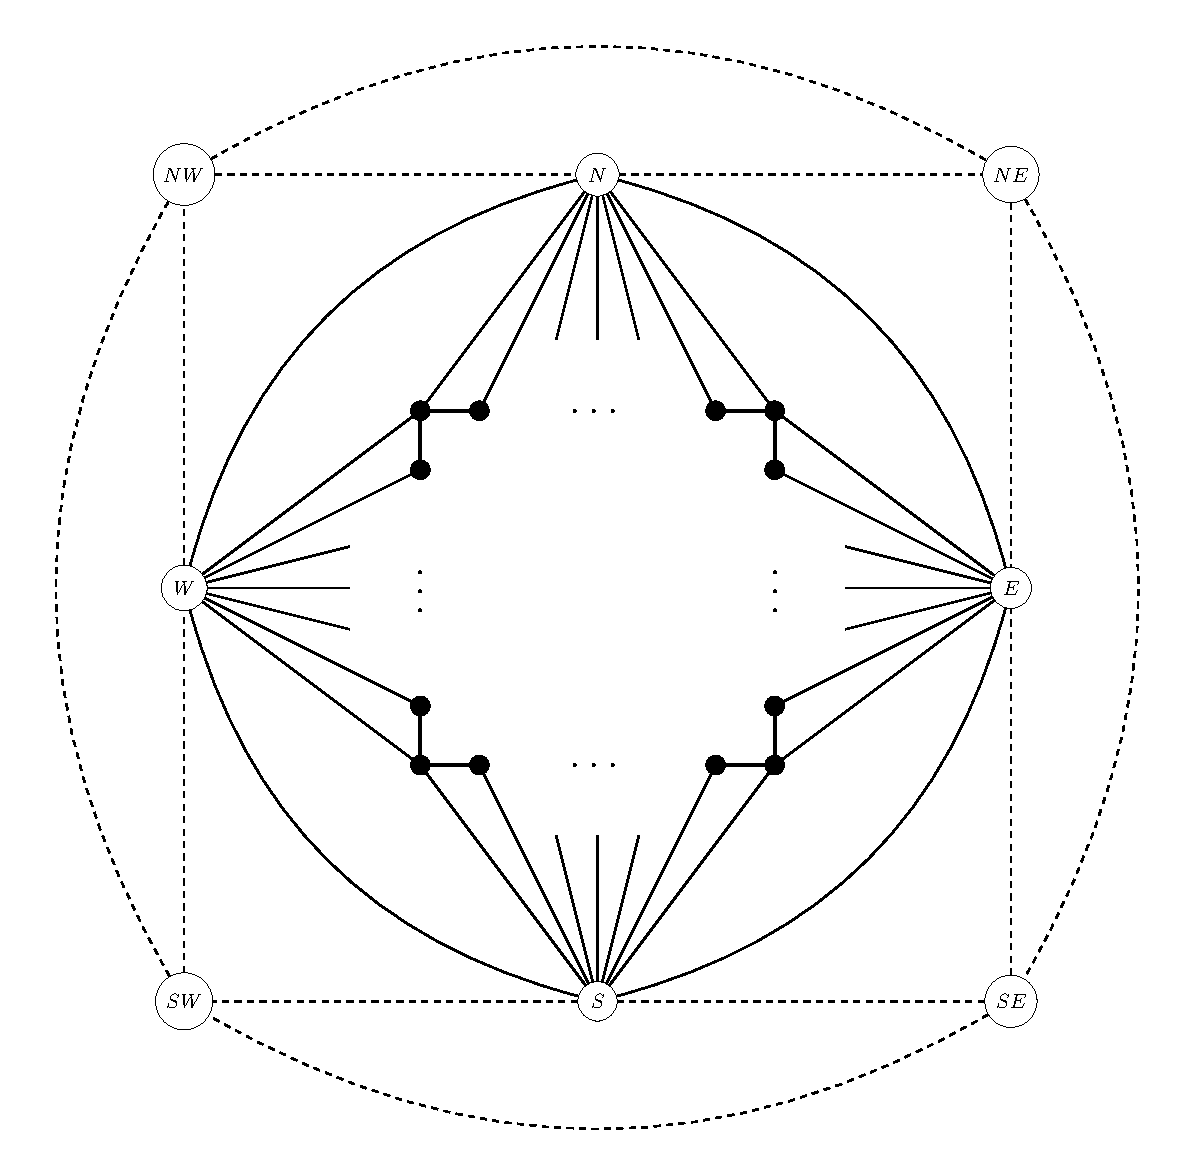
\includegraphics[scale=0.5]{img/scafold}

\caption{The construction of a scaffold. $G$ is displayed in thick lines and with closed vertices. An arbitrary extension $\ext G =H$ is then drawn with thin lines and open vertices. An extension of $H$ is then drawn with dashed edges and open vertices. 
    \label{fig:scafold}}
\end{figure}

The graph $H$ can have more then one extension but they all contain the separating $4$-cycle $\C= NESW$ thus by Lemma \ref{lem:fourCycleUnicolor} we see that, without loss of generality, the interior edges of $\C$ incident to $N$ and $S$ are coloured red and those incident to $E$ or $W$ are coloured blue. This is exactly as if we forced the extension $\ext G$

\subsection{An aplication: There are graphs that are $(2, \infty)$-sided}

We will show this by providing an example graph $G$ with a fixed extension $\ext G$ which we can do according to Theorem \ref{th:fixExtension}. Consider the graph in Figure \ref{fig:2manysidedLowerBound}. Note that most of the interior vertices are of degree $4$ and thus the largest part of any regular edge labelling is forced. Those edges that are forced to have a certain color are already coloured in Figure \ref{fig:2manysidedLowerBound}.


\begin{figure}[h!]
\centering
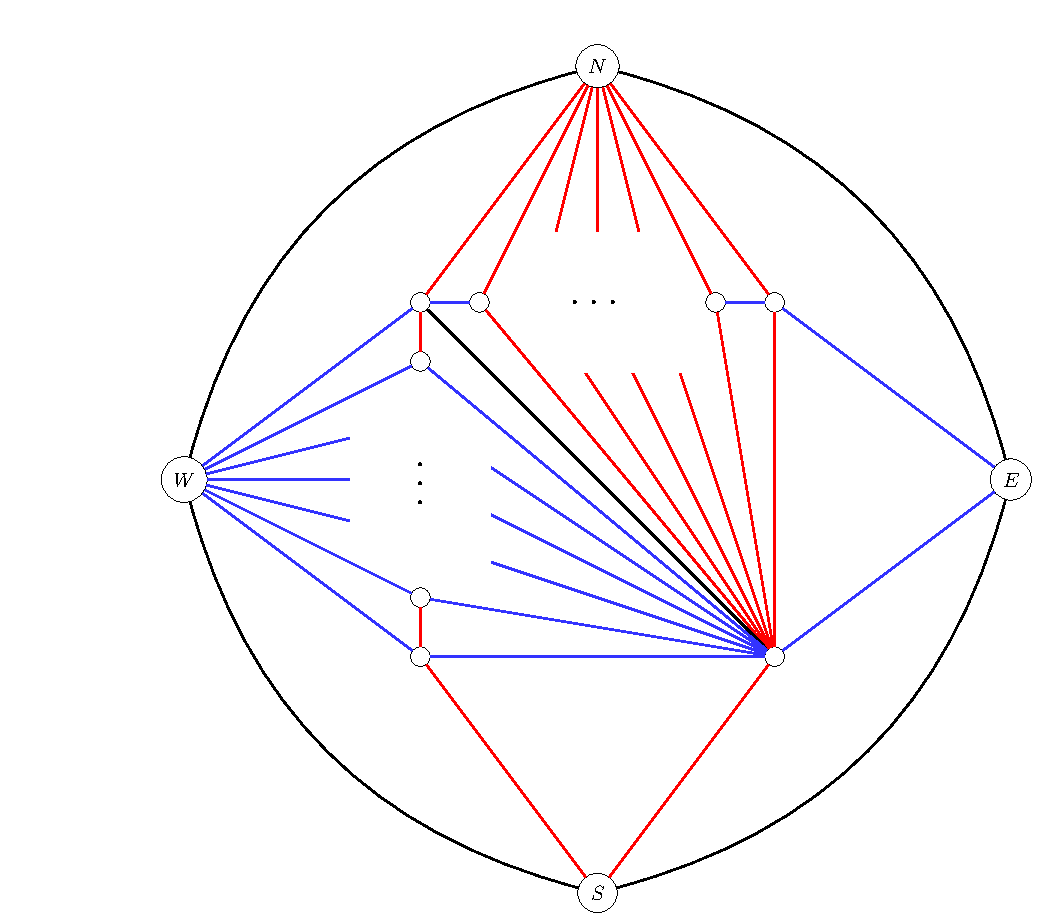
\includegraphics[scale=.5]{img/2manysidedLowerBound}

\caption{The fixed extension $\ext G$
    \label{fig:2manysidedLowerBound}}
\end{figure}

The only edge for which we have freedom to choose a color is the diagonal edge of $G$. Howeever, if we color this edge blue we get a red $(2, \infty)$ cycle and if we color this edge red we get a blue $(2, \infty)$ cycle. In both cases we will thus obtain a $(2,\infty)$-sided segment in our dual.




\end{document}
